
\subsection{Bionic end-effector}

Bionic prostheses is the closest a person with reduced functionality will come to a real arm.\\
In this chapter several options for bionic arms will be examined, to get a better understanding of the mechanics of the products on the market.\\

\subsubsection*{I-limb Ultra}

\begin{figure}[H]
    \centering
    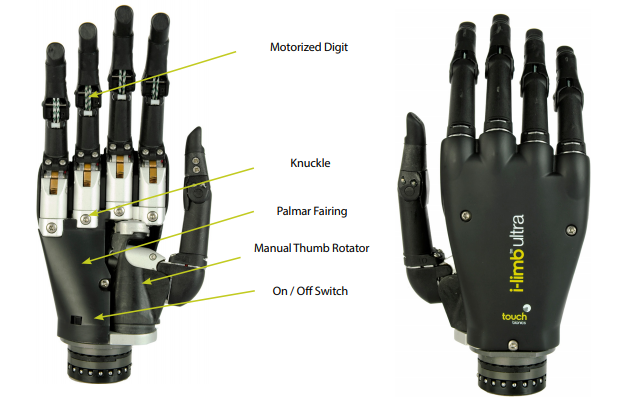
\includegraphics[width=12cm]{Figures/Contextual_figures/ProsthesesPics/i-limbultra.png}
    \caption{I-Limb Ultra\cite{I-limbUltra}}
    \label{fig:Ilimb-Ultra}
\end{figure}

The I-Limb Ultra device is an attachable bionic hand. It's flexible architecture allows the users to use both mobile application and muscles to signal the grip. These muscle signals are known as the myoelectric signals, and with the use from sensors in the patients residual limb, can allows the I-Limb to move as desired, while the app is for quick controls and specific grips.\\ 
The device has implemented proximity control administered by small Bluetooth devices, which triggers a grip when the the device is close to an object.\\
Gesture control is another feature offered by the "I-limb quantum". This allows the user to move the device in a certain direction to trigger a special and customised grip \cite{I-limbUltra}.
\\
%\begin{figure}[H]
%    \centering
%    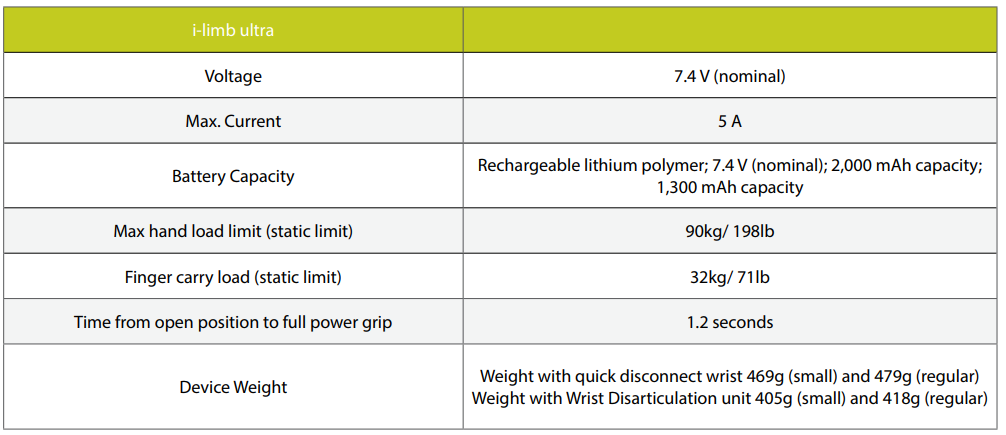
\includegraphics[width=15cm]{Figures/Contextual_figures/ProsthesesPics/specs.png}
%    \caption{I-Limb Ultra Specifications\cite{I-limbUltra}}
%    \label{fig:Ilimb-UltraSpecs}
%\end{figure}
\begin{table}[H]
    \centering
\begin{tabular}{ |P{7cm}||P{7.5cm}|  }
 \hline
 \multicolumn{2}{|c|}{I-limb ultra} \\
 \hline
 Voltage   & 7.4V (nominal)     \\
 \hline
 Max current &   5A  \\
 \hline
 Battery & Rechargeable lithium polymer 7.4V 2000 mAh  \\
 \hline
 Max hand load limit (static)    & 90kg \\
 \hline
 Finger carry load (static)& 32kg\\
 \hline
 Time from open position to full power grip & 1.2sec.  \\
 \hline
 Device weight  & Weight with quick disconnection wrist 469g(small size) and 479g(regular size)&&  Weight with wrist disarticulation unit 405g(small size) and 418g(regular size) \\
 \hline

\end{tabular}
\caption{Specification of I-limb ultra gripper}
    \label{tab:I-limb}
\end{table}
\subsubsection*{Be-Bionic}

\begin{figure}[H]
    \centering
    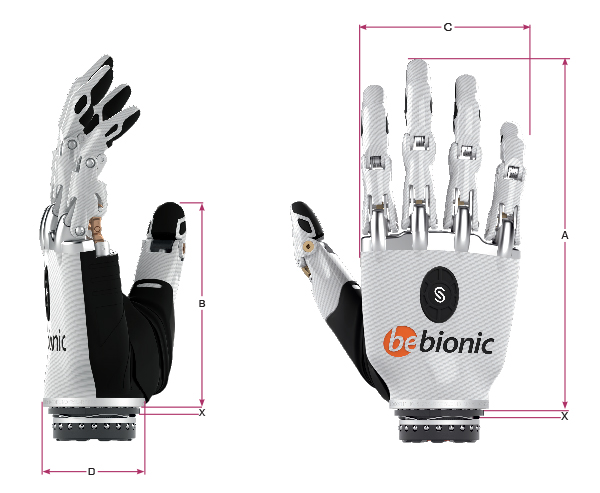
\includegraphics[width=10cm,height=7cm]{Figures/Contextual_figures/ProsthesesPics/Be-bionic.jpg}
    \caption{Be-Bionic \cite{Be-bionic}}
    \label{fig:Be-Bionic}
\end{figure}

The Be-Bionic hand takes advantage of multiple ergonomic features. The weight distribution of the motors in the hand makes the hand more comfortable to wear and feel lighter.\\
Balance software and microprocessors implemented in the hand, monitors the position and gives a more precise control.\\
Another useful feature is the auto grip, that ensures when items is slipping, the hand will then readjust to prevent this from happening.\\
\begin{table}[H]
    \centering
\begin{tabular}{ |P{7cm}||P{3cm}||P{3cm}|  }
 \hline
 \multicolumn{3}{|c|}{Be-Beonic} \\
 \hline
   & Large & Small \\
 \hline
 Maximum power grip force&140.1N&140.1N     \\
 \hline
 Maximum tripod grip force&36.6N&36.6N  \\
 \hline
 Maximum key grip force & 26.5N &26.5 \\
 \hline
 Maximum time to open or close -tripod grip &0.5 sec. &0.5 sec. \\
 \hline
  Maximum time to open or close - power grip & 1.0 sec. & 1.0 sec.\\
 \hline
  Maximum time to open or close - key grip & 1.0 sec. & 1.0 sec.  \\
 \hline
 Maximum static load - hook grip& 45 kg&45 kg\\
 \hline
  Maximum load individual fingers&25kg&25kg\\
  \hline
  Maximum finger tip extension load - hook grip&6kg&6kg\\
  \hline
   Maximum Safe vertical load taken through knuckles &90kg&90kg\\
   \hline
\end{tabular}
\caption{Specification of Be-Beonic gripper}
    \label{tab:Be-Beonic}
\end{table}
%\begin{figure}[H]
%    \centering
%    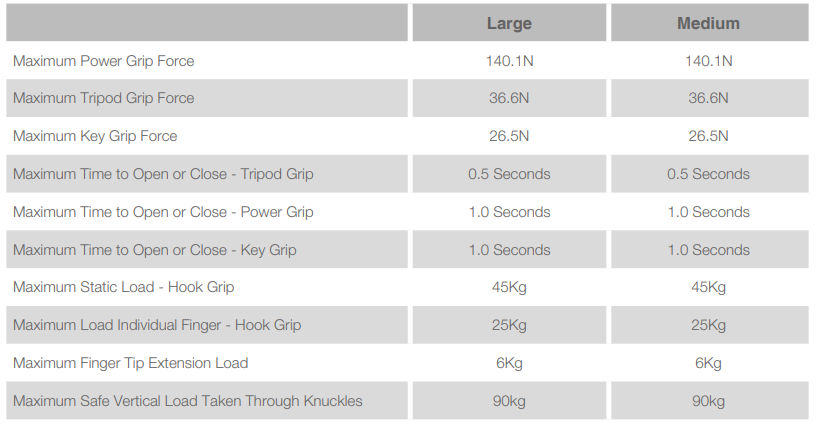
\includegraphics[width=15cm,height=6cm]{Figures/Contextual_figures/ProsthesesPics/specs-bebionic.png}
%    \caption{Be-Bionic Specifications \cite{Be-bionic}}
%    \label{fig:Be-BionicSpecs}
%\end{figure}
%\todo{set figure into excel}


\section{Conclusion}
When a user chooses a prostheses, there is several options and variables to consider. 
There is benefits and downsides to the different option, and as such, the user needs to figure out what function the prostheses needs to fulfil. 
If the goal is to avoid having to constantly deal with stares and awkward questions, then a Aesthetic prostheses would suffice. 
If added functionality such as added carrying capacity is required, then a mechanical option would be a better fit.
However as technology's becomes more advanced, it is also implemented into prostheses. These high tech solutions are very expensive, but also increases the users functionality as these have a higher amount of user control and can imitate the functionality of the human arm to an increasing degree.

For this project top help a user living with shoulder disarticulation in competing daily task, an electrical prostheses should be used. This prosthetic device must be operated with a control system which input is a surface EMG. \todo{several of the other control methods could also be used, maybe we should in the \textbf{Design} chapter mention that we will only look at EMG. instead of doing it here? }
The second control system interface which is chosen is the accelerometers and gyroscopes. Without these essential tools  the rotation and acceleration of the arm would be significantly harder to control.\\ \todo{we do this to increase our control options. because we only have 2 emg's. think this again should maybe be a delimitation}
The safety is established in such a way that the user cannot get harmed, the arm is placed on a table with Bluetooth connection, but requirements will be set up for this particular case later in the report.\\

both are viable,